%% Compiled with
% latexmk -pdfxe -pvc -shell-escape -silent slides.tex
%
% Use beamer + metropolis.
%
% In order to get the Fira font to work, xetex is required. Hence -pdfxe above.
%

%% TODO
% - determine projector aspect ratio; [aspectratio=1610] of beamer

%% Basic setup
\documentclass[xcolor={usenames,dvipsnames}]{beamer}
\usepackage[english]{babel}


%% NOTES, comment this for live slides
% \setbeameroption{show notes}


%% Use metropolis theme, with some custom settings
\usetheme[
  titleformat=smallcaps, % Font style of the title
  % numbering=fraction,
  progressbar=frametitle, % Add a progress bar under each slide title
  block=fill, % Make blocks actual blocks
]{metropolis}


%% Customise a few additional things
\setbeamertemplate{itemize items}[triangle]
\setbeamertemplate{caption}[default] % Prepend caption with "Figure" but no number
\setbeamertemplate{blocks}[rounded][shadow=true]


%% Don't count backup slides
\usepackage{appendixnumberbeamer}


% Extra colour definition
\definecolor{c1}{HTML}{006C71}
\definecolor{c2}{HTML}{005155}
\definecolor{c3}{HTML}{FF8928}
\definecolor{c4}{HTML}{E86900}
\colorlet{ImportantCode}{ForestGreen}
\colorlet{ImportantCode2}{RubineRed}
\colorlet{ImportantCode3}{RedOrange}


%% Use TikZ
\usepackage{tikz}
\usepackage{pgfplots}
\usetikzlibrary{shapes,fit,matrix,backgrounds,arrows,arrows.meta,positioning,chains,patterns,overlay-beamer-styles}
\tikzset{> = {Straight Barb[]}}


%% Use any font with XeTeX
\usepackage{fontspec}
\setmonofont[Contextuals={Alternate}]{Fira Code} % set font for tt (and minted)



%% Spacing
\usepackage{xspace}


%% Listings (using minted because listings has sever issues with beamer)
\usepackage{multicol}
\usepackage{minted}
\setminted{
  autogobble, % ignore leading spaces in code listings
  style=friendly,
  fontsize=\footnotesize,
}
\setmintedinline{
  % fontsize=\normalsize,
}


%% Custom commands
\newcommand{\GenC}{\emph{GenC}\xspace}
\newcommand{\QA}[2]{%
  \begin{flushleft}#1\end{flushleft}
  \pause
  \begin{flushright}#2\end{flushright}
}

\newcommand{\Inline}[1]{\texttt{#1}}
\newcommand{\InlineC}[1]{\mintinline{c}|#1|}
\newcommand{\InlineS}[1]{\mintinline{scala}|#1|}



%% Title Info
\title{Extending Safe C Support In Leon}
\date{February 2017}
\author{Marco Antognini}
\institute{Lab For Automated Reasoning And Analysis, EPFL}
\titlegraphic{\includegraphics[height=1cm]{res/epfl-logo.pdf}}



\begin{document}


%%%%%%%%%%%%%%%%%%%%%%%%%%%%%%%%%%%%%%%%%%%%%%%%%%%%%%%%%%%%%%%%%%%%%%%%%%%%%%%%%%%%%%%%%%%%%%%%%%%%%%%%%%%%%%%%%%%%%%%%
% Title & brief intro
\maketitle

\begin{frame}{Talk Overview}

  \GenC: safely converting Scala down to native C code.

  \vfill

  \begin{enumerate}
    \item Highlight of the key motivations for this work;
    \item What is Leon and why you want it to verify programs;
    \item Capabilities of \GenC through case studies;
    \item How MISRA compliance can be achieved.
  \end{enumerate}

\end{frame}



%%%%%%%%%%%%%%%%%%%%%%%%%%%%%%%%%%%%%%%%%%%%%%%%%%%%%%%%%%%%%%%%%%%%%%%%%%%%%%%%%%%%%%%%%%%%%%%%%%%%%%%%%%%%%%%%%%%%%%%%
% Motivation
%  - The world nowadays
%  - CVE, Overflows
%  - Critical systems: embedded, C, MUST BE crash-free
%  - Leon: verification, --genc
%  - Scala vs C: paradigms, runtime, contracts
\section{Motivation}

\begin{frame}{Software Nowadays}

  Hardware: more robust and efficient.

  {\hfill Solving a wider range of challenges.}

  \begin{center}
  \begin{tabular}{cc}
    \includegraphics[width=.2\textwidth]{res/curiosity.jpg} &
    \includegraphics[width=.2\textwidth]{res/robot.jpg} \\
    {\footnotesize Curiosity} & {\footnotesize BigDog} \\
    \includegraphics[width=.2\textwidth]{res/pacemaker.jpg} &
    \includegraphics[width=.2\textwidth]{res/road.jpg} \\
    {\footnotesize Pacemaker} & {\footnotesize Computer Vision}
  \end{tabular}
  \end{center}

  \begin{tikzpicture}[remember picture, overlay] % options needed to make reference to the page anchors.
    \node[anchor = south west, xshift = -0.75ex, yshift = 2em, rotate = 90] at (current page.south east) {
      \usebeamerfont{author in head/foot} \scriptsize Image Source: Wikimedia
    };
  \end{tikzpicture}
\end{frame}


\begin{frame}[standout]

  Fact:\\

  \alert{Software complexity} grows continuously.

  \pause \vfill

  What about the quality of software?

\end{frame}


\begin{frame}{CVE - Common Vulnerabilities and Exposures}

  \begin{figure}
  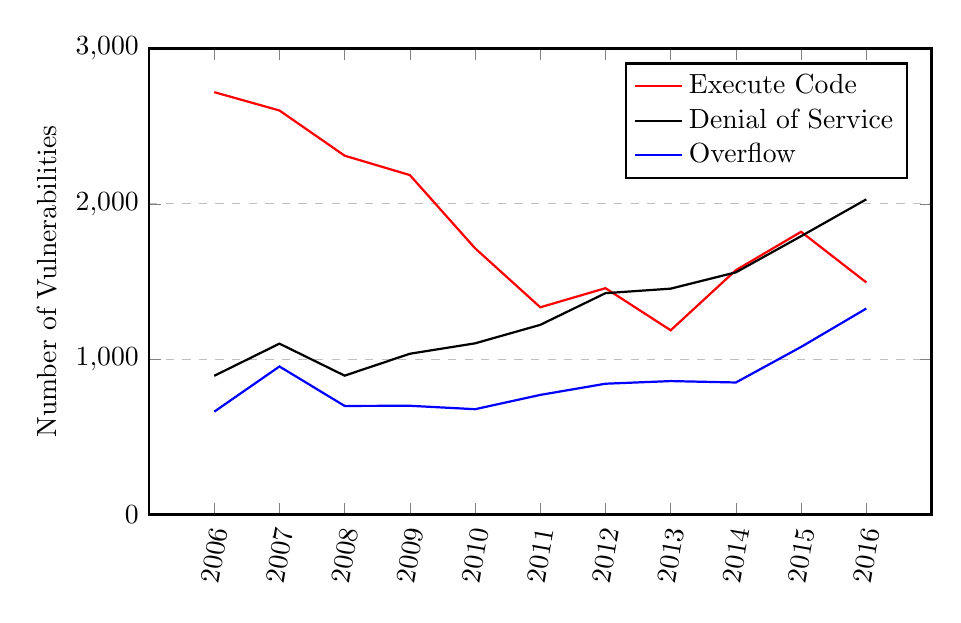
\begin{tikzpicture}
  \begin{axis}[
    % xlabel={Years}, % implicit enough to be hidden
    ylabel={Number of Vulnerabilities},
    ymin=0, ymax=3000,
    xtick={2006,2007,2008,2009,2010,2011,2012,2013,2014,2015,2016},
    xticklabel style={rotate=80},
    x tick label style={/pgf/number format/.cd,%
      scaled x ticks = false,
      set thousands separator={},
      fixed
    },
    xlabel shift=1pt,
    legend pos=north east,
    legend cell align=left,
    legend entries={Execute Code,Denial of Service,Overflow},
    ymajorgrids=true,
    grid style=dashed,
    width=0.95\textwidth,
    height=7.5cm,
    thick,
  ]

  \addplot[
    color=red,
    % mark=square,
    ]
    coordinates {%
    (2006,2719)(2007,2601)(2008,2310)(2009,2185)(2010,1714)(2011,1334)(2012,1457)(2013,1186)(2014,1573)(2015,1820)(2016,1494)
    };

  \addplot[
    color=black,
    % mark=circle,
    ]
    coordinates {%
    (2006,893)(2007,1100)(2008,894)(2009,1035)(2010,1102)(2011,1221)(2012,1425)(2013,1454)(2014,1559)(2015,1792)(2016,2029)
    };

  \addplot[
    color=blue,
    % mark=triangle,
    ]
    coordinates {%
    (2006,662)(2007,953)(2008,699)(2009,700)(2010,678)(2011,770)(2012,842)(2013,859)(2014,850)(2015,1079)(2016,1326)
    };

  \end{axis}
  \end{tikzpicture}
  \vspace{-2.1ex}
  \caption{The 3 most frequent categories of bugs in the last 10 years.}
  \end{figure}

  \begin{tikzpicture}[remember picture, overlay] % options needed to make reference to the page anchors.
    \node[anchor = south west, xshift = -0.75ex, yshift = 2em, rotate = 90] at (current page.south east) {
      \usebeamerfont{author in head/foot} \scriptsize Source: \; \url{cve.mitre.org} \; \& \; \url{cvedetails.com}
    };
  \end{tikzpicture}

\end{frame}


\begin{frame}{CVE - Common Vulnerabilities and Exposures (cont.)}

  Credibility of the data?

  \begin{block}{Some numbers:}

    \begin{description}[Integer Overflowsx] % make sure there's an extra char for the margin look

      \item[Life Span]         Since 1999
      \item[Tickets]           Over 80k (4k-8k by year in the last decade)
      \item[Actors]            Adobe, Apache, Apple, Cisco, Google,\\
                               Linux, Microsoft, Mozilla, ...

    \end{description}

  \end{block}

  \pause

  \begin{block}{\emph{Overflows} are trending!}

    \begin{description}[Integer Overflowsx] % same as above

      \item[Ranking by type]   Overflows are third
      \item[Integer Overflows] $\sim 1.6\%$ of total tickets
      \item[Buffer Overflows]  \alert{$\sim 10\%$} of total tickets

    \end{description}

  \end{block}

\end{frame}


\begin{frame}{Critical Systems}

  \begin{block}{Challenges}

    \begin{enumerate}
      \item \textbf{No Failure Can Be Tolerated} (injury, death, money loss, ...)
      \item \textbf{Embedded Devices} (spacecrafts, cars, medical implants, ...)
      \item \textbf{Low Level Programming} (usually in C)
    \end{enumerate}

  \end{block}

  \pause \vfill

  \begin{block}{Addressing the challenges}

    \begin{enumerate}
      \item \textbf{Verification \& certification};
      \item Precise requirements for hardware;
      \item Open question; C is known to be tricky.
    \end{enumerate}

  \end{block}

\end{frame}


\begin{frame}[fragile]{C: Some Pitfalls}

  \begin{minted}{c}
  int k = i << j; // when is this safe?
  \end{minted}

  \pause

  \begin{itemize}
    \item Range of \InlineC{int}?
    \item Representation of \InlineC{int}?
    \item Value of \InlineC{j}?
    \item If \InlineC{i} is signed, is \InlineC{i << j} representable?
    \item Possible type cast and UB on assignment.
    \item ...
  \end{itemize}

\end{frame}


\begin{frame}[fragile]{Certification: \alert{MISRA} Guidelines for C}

  \note<1>{dynamic alloc = DANGER 2x (memory limit + unpredictable latency)}

  {\hfill \emph{Motor Industry Software Reliability Association}}
  \vfill

  Make C safer through a set of directives that:
  \begin{itemize}

    \item Put emphasis on \emph{best practices};
    \item Avoid triggering undefined, unspecified or implementation-defined behaviour;
    \item Restrict the language {\footnotesize(e.g. \alert{no dynamic allocation}, parts of \emph{SL}, ...);}
    \item Recommend specific arithmetic types \& operations.
    % \item Indirectly promote usage of \alert{static analysers}.

  \end{itemize}

\end{frame}


\begin{frame}[standout]

  \note<1>[item]{MISRA == Plaster, it protects but doesn't heal.}
  \note<1>[item]{Writing C helps: many compilers already available.}

  \QA{Do we have to write C code when targeting embedded devices?}{\emph{Yes and No.}}
  \pause \vfill

  \QA{Couldn't we write Scala code instead?}{Spoiler Alert: \emph{Yes!}}
  \pause \vfill

  \QA{Can we detect overflows at compile time?}{\emph{Yes.}}%, but...}}

\end{frame}



%%%%%%%%%%%%%%%%%%%%%%%%%%%%%%%%%%%%%%%%%%%%%%%%%%%%%%%%%%%%%%%%%%%%%%%%%%%%%%%%%%%%%%%%%%%%%%%%%%%%%%%%%%%%%%%%%%%%%%%%
% Leon & GenC
%  - dev pipeline
%  - new features for Leon itself
%  - what GenC is: a transpiler with MISRA in mind
%  - features overview
\section{Leon \& \GenC}

\begin{frame}[fragile]{Writing Safe Code With \alert{Leon}}

  \note<1>{Contract programming in Scala and verify contracts with Leon.}

  \begin{center}
  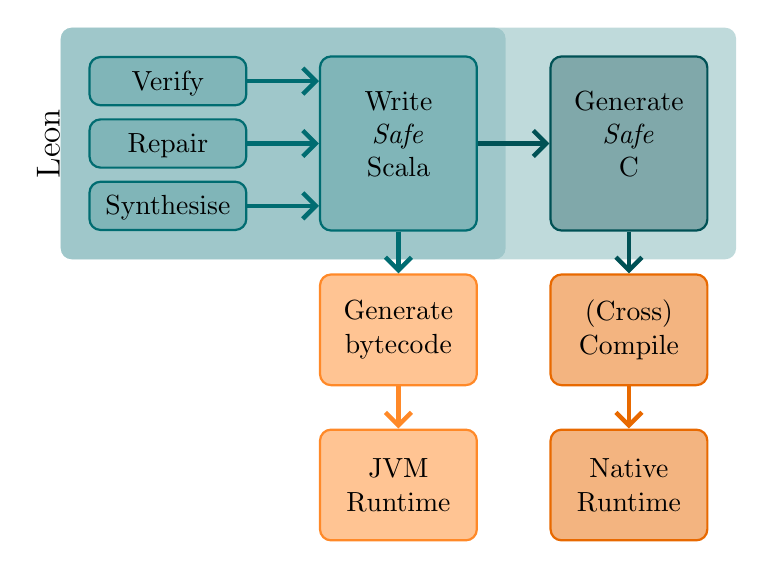
\begin{tikzpicture}
    [auto,
     commonbox/.style = {
       rectangle, draw = #1, thick, fill = #1!50,
       text width = 5em, text centered, rounded corners,
     },
     phantom1/.style = {
       text depth = .5ex, text height = 2ex,
     },
     phantom2/.style = {
       % text depth = .5ex, text height = 5ex,
       align = center, anchor = center,
       minimum height = 4em,
     },
     box1/.style = {
       commonbox = #1,
       phantom1,
     },
     box2/.style = {
       commonbox = #1,
       phantom2,
     },
    ]

    \matrix (m) [%
      column sep = 6ex, row sep = 1ex,
      matrix of nodes,
      nodes in empty cells,
      nodes = { }, %text depth = .5ex, text height = 2ex },
    ] {%
      |[box1 = c1]| {Verify}     & |[phantom1]|                      & |[phantom1]|                                        \\
      |[box1 = c1]| {Repair}     & |[phantom1]|                      & |[phantom1]|                                        \\
      |[box1 = c1]| {Synthesise} & |[phantom1]|                      & |[phantom1]|                                        \\
      && \\ % empty line for spacing
      |[phantom2]|               & |[box2 = c3]| {Generate bytecode} & |[box2 = c4, visible on = <2>]| {(Cross)\\ Compile} \\
      && \\ % empty line for spacing
      |[phantom2]|               & |[box2 = c3]| {JVM Runtime}       & |[box2 = c4, visible on = <2>]| {Native Runtime}    \\
    };

    \node [fit = (m-1-2)(m-3-2), commonbox = c1, inner ysep = 0em]                   (scala) {Write\\ \emph{Safe}\\ Scala};
    \node [fit = (m-1-3)(m-3-3), commonbox = c2, inner ysep = 0em, visible on = <2>] (genc)  {Generate\\ \emph{Safe}\\ C};

    \begin{scope}[every node/.style={font=\small\itshape}, ultra thick, ->]
      \begin{scope}[c1]
        \draw (m-1-1.east) to (m-1-1-|scala.west);
        \draw (m-2-1.east) to (m-2-1-|scala.west);
        \draw (m-3-1.east) to (m-3-1-|scala.west);
        \draw (scala.south) to (m-5-2.north);
      \end{scope}
      \draw [c3] (m-5-2.south) to (m-7-2.north);

      \begin{scope}[visible on = <2>]
        \draw [c2] (scala.east) to (genc.west);
        \draw [c2] (genc.south) to (m-5-3.north);
        \draw [c4] (m-5-3.south) to (m-7-3.north);
      \end{scope}
    \end{scope}

    \begin{pgfonlayer}{background}
      \node[fill=c1!50,opacity=.5,inner sep=10pt,rectangle,rounded corners,
            fit=(m-1-1) (scala), visible on = <1>] (leon) {};
      \node[fill=c1!50,opacity=.5,inner sep=10pt,rectangle,rounded corners,
            fit=(m-1-1) (genc), visible on = <2>] {};
      \node[font=\large, anchor = center, rotate = 90, yshift = 1ex] at (leon.west) {Leon};
    \end{pgfonlayer}
  \end{tikzpicture}
  \end{center}
  % \caption{Development Process}

\end{frame}


\begin{frame}[fragile]{Programming By Contract: Example A}

  \note{pre-, postconditions represent the contracts}

  \begin{minted}[highlightlines={2,4}]{scala}
def clamp(x: Int, down: Int, up: Int): Int = {
  require(down <= up)
  max(down, min(x, up))
} ensuring { res => inRange(res, down, up) }
  \end{minted}

\end{frame}


\begin{frame}[fragile]{Programming By Contract: Example B}

  \note{precondition \& loop invariant; illustrate I/O}

  \begin{minted}[highlightlines={3,12}]{scala}
def skipBytes(fis: leon.io.FileInputStream, count: Int)
             (implicit state: leon.io.State): Boolean = {
  require(fis.isOpen && 0 <= count)

  var i = 0
  var success = true

  (while (success && i < count) {
    val opt = fis.tryReadByte()
    success = opt.isDefined
    i += 1
  }) invariant (inRange(i, 0, count))

  success
}
  \end{minted}

\end{frame}


\begin{frame}[fragile]{New Verification Features For Leon}

  \begin{itemize}
    \item Support for \InlineS{Byte} and integer cast operations.
    \item More \Inline{--overflow} checking:
      \begin{itemize}
        \item \InlineS{-Int.MinValue}
        \item \InlineS{Int.MinValue / -1}
      \end{itemize}
    \item \Inline{--strict-arithmetic} checking:
      \begin{itemize}
        \item Right hand side of \InlineS{<< >> >>>} must be in $[0, 31]$;
        \item \InlineS{Int.MinValue} \texttt{\%} \InlineS{-1} undefined in C.
      \end{itemize}
    \item Safe I/O API:
      \begin{itemize}
        \item Provide interface for \InlineC{[f]printf} and \InlineC{[f]scanf}.
      \end{itemize}
  \end{itemize}

\end{frame}


\begin{frame}[fragile]{\GenC}

  \hspace*{-2.75em}
  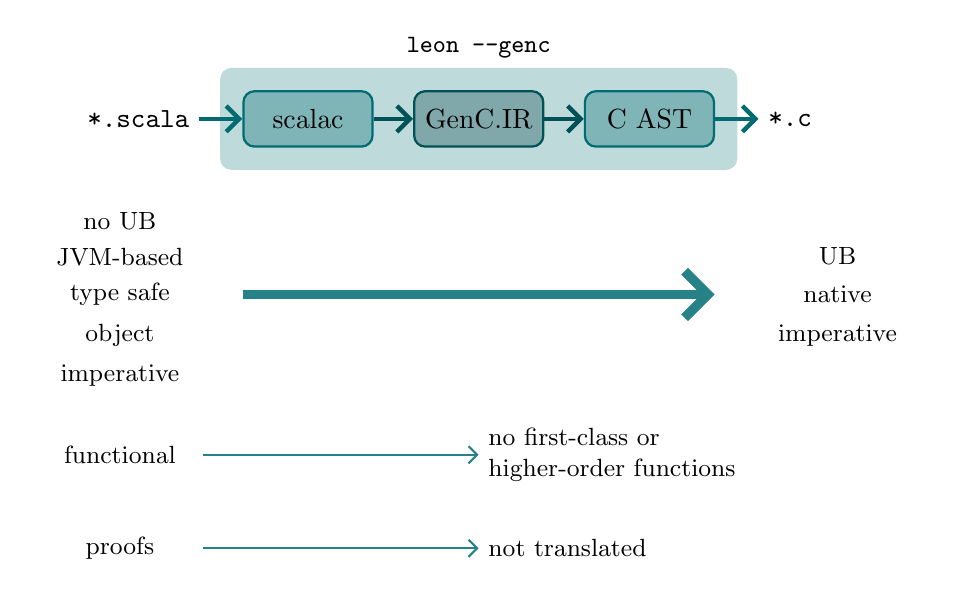
\begin{tikzpicture}
    [auto,
     second/.style = {
       visible on = <2>,
     },
     box/.style = {rectangle, draw=#1, thick, fill=#1!50,
                   text width=4em, text centered, rounded corners,
                   minimum height=2em},
     bla/.style = {font=\small, minimum width = 6em, second},
     file/.style = {text width = 5em},
     arggg/.style = {text width = 4em},
    ]

    \matrix [column sep=5mm,row sep=0mm]
    {%
      % row 1
      \node [file]   (source)     {\hfill\Inline{*.scala}}; &
      \node [box=c1] (compile)    {scalac};                 &
      \node [box=c2] (ir)         {GenC.IR};                &
      \node [box=c1] (cast)       {C AST};                  &
      \node [file]   (output)     {\Inline{*.c}\hfill};     \\

      \node [minimum height=2em] {}; &&&& \\ % vertical space

      \node [bla] (scala0) {no UB};         &&&&                                        \\
      \node [bla] (scala1) {JVM-based};     &&&& \node [bla] (c990) {UB};               \\
      \node [bla] (scala2) {type safe};     &
                \node [arggg] (anchor0) {}; && \node [arggg] (anchor1) {};
                                            &    \node [bla] (c991) {native};           \\
      \node [bla] (scala3) {object};        &&&& \node [bla] (c992) {imperative};       \\
      \node [bla] (scala4) {imperative};    &&&&                                        \\

      \node [minimum height=1.5em] {}; &&&& \\ % vertical space

      \node [bla] (scala5) {functional};    && \node (ns) {}; && \\

      \node [minimum height=2em] {}; &&&& \\ % vertical space

      \node [bla] (scala6) {proofs};        && \node (nt) {}; && \\
    };

    \begin{scope}[every node/.style={font=\small\itshape}, ultra thick, ->]
      \draw [c1] (source.east)  to (compile.west);
      \draw [c2] (compile.east) to (ir.west);
      \draw [c2] (ir.east)      to (cast.west);
      \draw [c1] (cast.east)    to (output.west);
    \end{scope}

    \begin{scope}[second]
      \draw[->, c1!85, line width = 0.8ex] (anchor0.west) to (anchor1.east);

      \draw (ns.base) node[bla, anchor = west, text width = 15em] (nst) {no first-class or\\ higher-order functions};
      \draw (nt.base) node[bla, anchor = west, text width = 15em] (ntt) {not translated};
      \draw[->,thick, c1!85] (scala5.east) to (nst.west);
      \draw[->,thick, c1!85] (scala6.east) to (ntt.west);
    \end{scope}

    \begin{pgfonlayer}{background}
      \node[fill=c1!50,opacity=.5,inner sep=8pt,rectangle,rounded corners,
            fit=(compile) (cast)] (leon) {};
          \node[above, font=\small] at (leon.north) {\Inline{leon --genc}};
    \end{pgfonlayer}
  \end{tikzpicture}

\end{frame}


\begin{frame}{\GenC: Memory Model}

  \begin{block}{Mutability}
    JVM References \Inline{===} C Pointers.

    \textbf{No Aliasing} \Inline{==>} 1 owner of memory, deterministic lifetime.
  \end{block}

  \vfill

  \begin{block}{Allocation}
    \textbf{No dynamic memory allocation}.

    % Every variable has a single \emph{allocation point}.

    % Exception: arrays.
  \end{block}

\end{frame}


\begin{frame}[fragile]{\GenC: Supported Types}
  \begin{itemize}
    \item Basic types \& (ASCII) literals:\\
          \InlineS{Unit Boolean Byte Int Char String}
    \item \InlineS{Arrays[T]}: stack-allocated, \alert{can't be returned}.
    \item \InlineS{TupleN[T1, ..., TN]}.
    \item Classes:
      \begin{itemize}
        \item \InlineS{case class}, with mutable \InlineS{var} fields;
        \item Generics {\small (no type erasure in Leon)};
        \item Inheritance with \emph{tagged-union};
        \item ``Enumeration'' \InlineC{==> enum};
        \item \alert{No recursive types}, e.g. \InlineS{List};
        \item External types: \InlineS{@cCode.typdef(alias, include)}.
      \end{itemize}
  \end{itemize}
\end{frame}


\begin{frame}{\GenC: Supported Functions}
  \begin{itemize}
    \item Top-level or nested function;
    \item Free or member function;
    \item Generic or regular function;
    \item Overloaded or unique function;
    \item \alert{No higher-order function};
    \item External function: \InlineS{@cCode.function(code, includes)}.
  \end{itemize}
\end{frame}


\begin{frame}[fragile]{\GenC: Supported Expressions}
  \begin{itemize}
    \item Control flow: \InlineS{if-else}, \InlineS{while}, \& pattern matching;
    \item Membership test \& cast for object;
    \item Function call;
    \item Array access \& update;
    \item Arithmetic operation:
      \begin{itemize}
        \item Mimicking Java operators \& integer promotion rules.
        \item \mintinline{scala}{+ - * / % & | ~ ^ && || << >>>}
      \end{itemize}
    \item \alert{Normalised} execution order.
  \end{itemize}
\end{frame}



%%%%%%%%%%%%%%%%%%%%%%%%%%%%%%%%%%%%%%%%%%%%%%%%%%%%%%%%%%%%%%%%%%%%%%%%%%%%%%%%%%%%%%%%%%%%%%%%%%%%%%%%%%%%%%%%%%%%%%%%
% Case Studies:
%  - LZW
%  - Image Processing
\section{Case Studies}

\begin{frame}{LZW: Overview}

  \begin{block}{Goal}
    \begin{enumerate}
      \item Load/save file (binary I/O),
      \item Compress/decompress data with a fixed amount of memory (based on dictionary manipulation).
    \end{enumerate}
  \end{block}

\end{frame}


\begin{frame}{LZW: Results}

  \begin{itemize}
    \item Strings of \InlineS{Byte} are represented using fixed-size \InlineS{Buffer}s.
    \item Two implementations of \InlineS{Dictionary}:
      \begin{enumerate}
        \item[A.] \InlineS{Dictionary} $\approx$ \InlineS{Array[Buffer]} (nested arrays),
        \item[B.] \InlineS{Dictionary} $\approx$ \InlineS{Array[Byte]}\;\;\;\: (one array only).
      \end{enumerate}
    \item A. is \emph{DRY} \& faster but takes significantly more time to compile and uses more memory at runtime.
    \item Runtime bottleneck: dictionary lookup complexity.
  \end{itemize}

\end{frame}

\begin{frame}{Image Processing: Overview}

  \begin{block}{Goal}
    \begin{enumerate}
      \item Load BMP file (I/O, parsing),
      \item Apply some kernel (matrix convolution) onto the image,
      \item Save the resulting image as BMP (more I/O, conversion).
    \end{enumerate}
  \end{block}

\end{frame}


\begin{frame}[fragile]{Image Processing: Using Kernels}
  \begin{minted}{scala}
    // Sharpen
    val kernel = Kernel(size = 5, scale = 25, Array(
      -1, -1, -1, -1, -1,
      -1,  2,  2,  2, -1,
      -1,  2,  8,  2, -1,
      -1,  2,  2,  2, -1,
      -1, -1, -1, -1, -1
    ))

    def processImage(src: Image): Status = {
      val dest = createImage(src.w, src.h)
      kernel.apply(src, dest)
      saveImage(fos, dest)
    }
  \end{minted}
\end{frame}


\begin{frame}[fragile]{Image Processing: Kernels}

  \begin{center}
    \begin{tikzpicture}[->, thick, c2, auto]
      \matrix[row sep = 1mm, column sep = 3cm]{
        \node (i0) {\includegraphics[width = .2\textwidth]{res/input3.png}};        &
        \node (o0) {\includegraphics[width = .2\textwidth]{res/output3edge.png}};   \\
        \node (i1) {\includegraphics[width = .2\textwidth]{res/input2.png}};        &
        \node (o1) {\includegraphics[width = .2\textwidth]{res/output2blur3x.png}}; \\
        \node (i2) {\includegraphics[width = .2\textwidth]{res/input6.png}};        &
        \node (o2) {\includegraphics[width = .2\textwidth]{res/output6sharp.png}};  \\
      };

      \path (i0) edge node {edge detection} (o0);
      \path (i1) edge node {blurring}       (o1);
      \path (i2) edge node {sharpening}     (o2);
    \end{tikzpicture}
  \end{center}

  All outputs are produced through Leon/\GenC.

\end{frame}



%%%%%%%%%%%%%%%%%%%%%%%%%%%%%%%%%%%%%%%%%%%%%%%%%%%%%%%%%%%%%%%%%%%%%%%%%%%%%%%%%%%%%%%%%%%%%%%%%%%%%%%%%%%%%%%%%%%%%%%%
% MISRA
\section{MISRA: Working Toward Compliance}

\begin{frame}{Defining a Standard C Environment}

  \begin{exampleblock}{Directive 1.1}
    Any implementation-defined behaviour on which the output of the program depends shall be documented and understood.
  \end{exampleblock}

  % \begin{exampleblock}{Directive 4.2}
  %   All usage of assembly language should be documented.
  % \end{exampleblock}

  % \begin{exampleblock}{Directive 4.3}
  %   Assembly language shall be encapsulated and isolated.
  % \end{exampleblock}

  % \begin{exampleblock}{Rule 1.1}
  %   The program shall contain no violations of the standard C syntax and
  %   constraints, and shall not exceed the implementation’s translation limits.
  % \end{exampleblock}

  % \begin{exampleblock}{Rule 1.2}
  %   Language extensions should not be used.
  % \end{exampleblock}

  % \begin{exampleblock}{Rule 1.3}
  %   There shall be no occurrence of undefined or critical unspecified behaviour.
  % \end{exampleblock}

  \pause

  \begin{block}{Requirements for the \alert{C99} implementation}
    \begin{itemize}
      \item The availability of \InlineC{int8_t}, \InlineC{int32_t} and \InlineC{uint32_t} types;
      \item Converting \InlineC{int32_t <-> uint32_t} works as expected;
      \item A \emph{byte} has 8 bits;
      \item No other language extensions or requirements,
      \item No use of assembly instructions.
    \end{itemize}
  \end{block}

  % \begin{center} Assuming \Inline{--strict-arithmetic}. \end{center}

\end{frame}


\begin{frame}{Limiting Runtime Errors}

  \begin{exampleblock}{Directive 4.1}
    Run-time failures shall be minimized.
  \end{exampleblock}

  % \begin{exampleblock}{Directive 4.11}
  %   The validity of values passed to library functions shall be checked.
  % \end{exampleblock}

  \pause

  \begin{block}{Avoiding runtime errors}
    \begin{enumerate}
      \item \emph{Arithmetic errors} are detected with {\footnotesize\Inline{--strict-arithmetic}};
      \item \emph{Pointer arithmetic} is not used;
      \item \emph{Function contract violations} and
      \item \emph{Array overflows} are detected when verifying the code;
      \item \emph{Pointers dereferencing} are safe under our memory model;
      \item No \emph{dynamic memory allocations} are used.
    \end{enumerate}
  \end{block}

\end{frame}


\begin{frame}[fragile]{Rule Subsumed Under Verification: Array Overflows}

  % Several of MISRA directives can be ensured through verification.

  \begin{exampleblock}{Rule 18.1}
    A pointer resulting from arithmetic on a pointer operand shall address an
    element of the same array as that pointer operand.
  \end{exampleblock}

  \pause

  \begin{columns}
    \begin{column}{0.3\textwidth}
      \begin{minted}[xleftmargin = -4.5ex]{scala}
        def swap(data: Array[Int],
                 i: Int, j: Int) {
          val tmp = data(i)
          data(i) = data(j)
          data(j) = tmp
        }
      \end{minted}
    \end{column}
    \begin{column}{0.6\textwidth}
      \pause
      \begin{minted}{c}
        static void swap_0(array_int32 data_0,
                    int32_t i_3, int32_t j_0) {
          int32_t tmp_0 = data_0.data[i_3];
          data_0.data[i_3] = data_0.data[j_0];
          data_0.data[j_0] = tmp_0;
        }
      \end{minted}
    \end{column}
  \end{columns}

  \pause

  \begin{alertblock}{Example of Verification Report}
    \centering \includegraphics[width=0.7\textwidth]{res/verification_error.png}
  \end{alertblock}

  % \begin{itemize}
  %   \item All functions return (i.e. exhaustive patter matching)
  %   \item Division by zero, arithmetic overflows, rhs of shifts, ...
  %   \item Function call , ......
  % \end{itemize}

  % \begin{minted}{scala}
  % def normdot(a: Array[Int], b: Array[Int]): Int = {
  %   var sum = 0
  %   var i = 0
  %   while (i < a.length) {
  %     sum += a(i) * b(i) // overflow + invalid access
  %     i += 1
  %   }
  %   sum / a.length // division by zero
  % }
  % \end{minted}

\end{frame}


\begin{frame}{Other Considerations}

  Verification identifies potential problems before execution.% (6)

  \GenC carefully crafts the C code to respect many rules.% (26)

  % Some minor rules are not fulfilled. (5)

  \pause \vfill

  But \GenC does not claim to replace MISRA:
  \begin{itemize}
    \item Function results should be used;
    \item There should be no unreachable or dead code;
    \item Recursive functions should be avoided;
    % \item VLA and I/O should not be used;
    \item ...
  \end{itemize}

  {\hfill 20 rules are left to the user of the 159 overall rules.}

\end{frame}



%%%%%%%%%%%%%%%%%%%%%%%%%%%%%%%%%%%%%%%%%%%%%%%%%%%%%%%%%%%%%%%%%%%%%%%%%%%%%%%%%%%%%%%%%%%%%%%%%%%%%%%%%%%%%%%%%%%%%%%%
% Conclusion
\section{Conclusion}

\begin{frame}{Summary}

  \begin{itemize}
    \item More verification tools for Leon.
      \vfill
      % \begin{itemize}
      %   \item \InlineS{Byte},
      %   \item strict arithmetic checking,
      %   \item I/O API.
      % \end{itemize}
    \item A significant fragment of Scala \alert{safely} translatable to C.
      \vfill
    \item A simple memory model is possible when no aliasing.
      \vfill
    \item Most of MISRA is guaranteed to be satisfied.
      \vfill
    \item Case studies showed we can write software with \GenC!
  \end{itemize}

\end{frame}


\begin{frame}{Future Works -- Beside \GenC Itself}

  \begin{block}{MISRA}
    Linter: warn user about (more) rule violations.
  \end{block}

  \begin{block}{Performance: HashMap Case Study}
    Scala vs C comparison.
  \end{block}

  \begin{block}{Resource Inference}
    Combine \GenC and Orb to infer memory \& time metrics.
  \end{block}

  \begin{block}{More Numerical Types \& Libraries}
    \InlineS{Short}, \InlineS{Long}, \InlineS{FixedPoint}, \InlineS{ArrayList}, ...
  \end{block}

\end{frame}



%%%%%%%%%%%%%%%%%%%%%%%%%%%%%%%%%%%%%%%%%%%%%%%%%%%%%%%%%%%%%%%%%%%%%%%%%%%%%%%%%%%%%%%%%%%%%%%%%%%%%%%%%%%%%%%%%%%%%%%%
% Questions
\begin{frame}[standout]
  \Huge Thank You!
\end{frame}



%%%%%%%%%%%%%%%%%%%%%%%%%%%%%%%%%%%%%%%%%%%%%%%%%%%%%%%%%%%%%%%%%%%%%%%%%%%%%%%%%%%%%%%%%%%%%%%%%%%%%%%%%%%%%%%%%%%%%%%%
% Backup Slides
\appendix

\begin{frame}[standout]
  % Empty slide.
\end{frame}

% TODO
%   - Why List is not possible through an example.

\begin{frame}{LLVM IR vs C}

  Why C99 was chosen? \vspace{-1ex}
  \begin{itemize}
    \item C is widely used;
    \item Many compilers for C for many hardware architectures;
    \item Prior experience in C;
    \item MISRA ``compatible''.
  \end{itemize}

  \vfill

  Is LLVM IR a good alternative? \vspace{-1ex}
  \begin{itemize}
    \item Probably yes: getting popular;
    \item MISRA principles could be ``translated'';
    \item Lower level means more opportunity for optimisation;
    \item Probably more strictly defined than C.
  \end{itemize}

\end{frame}


\begin{frame}{Language Shares}
  \begin{figure}
    \includegraphics[width=\textwidth]{res/saks.embedded.languages.shares.png}
  \end{figure}
  \hfill \tiny \url{https://youtu.be/D7Sd8A6_fYU}
\end{frame}


\begin{frame}[fragile]{Programming By Contract: Example A, Fixed}

  \begin{minted}[highlightlines={6}]{scala}
    def clamp(x: Int, down: Int, up: Int): Int = {
      require(down <= up)
      max(down, min(x, up))
    } ensuring { res =>
      inRange(res, down, up) &&
      (inRange(x, down, up) ==> (res == x))
    }
  \end{minted}

\end{frame}



%%%%%%%%%%%%%%%%%%%%%%%%%%%%%%%%%%%%%%%%%%%%%%%%%%%%%%%%%%%%%%%%%%%%%%%%%%%%%%%%%%%%%%%%%%%%%%%%%%%%%%%%%%%%%%%%%%%%%%%%
% Support Features
\section{Supported Features}

\begin{frame}[fragile]{Basic Types}

  \begin{itemize}

    \item Basic Types:\\
      \begin{tabular}{llllll}
        \InlineS{Unit} & \InlineS{Boolean} & \InlineS{Byte}   & \InlineS{Int}     & \InlineS{Char} & \InlineS{String} \\
        \InlineC{void} & \InlineC{bool}    & \InlineC{int8_t} & \InlineC{int32_t} & \InlineC{char} & \InlineC{char*}
      \end{tabular}

    \item And their respective literals\footnote{ASCII literals only}.

  \end{itemize}

\end{frame}


\begin{frame}[fragile]{Arrays}

  \begin{itemize}

    \item \InlineS{Array[T]} is mapped into
      \begin{minted}{c}
      typedef struct { T* data; int32_t length; }
              array_T;
      \end{minted}

    \pause

    \item An array needs two \emph{allocation points}:\\
      \begin{minted}{scala}
      val a = Array(0, 1, 2, 3)
      \end{minted}
      is translated into
      \begin{minted}{c}
      int32_t leon_buffer_0[4] = { 0, 1, 2, 3 };    // (1)
      array_int32 a = (array_int32) {               // (2)
        .data = leon_buffer_0, .length = 4
      };
      \end{minted}

    \pause

    \item \alert{Stack-allocated arrays cannot be returned from functions!}

    \item \emph{Variable Length Array} (VLA) are supported with a warning.

  \end{itemize}

\end{frame}


\begin{frame}[fragile]{Case Classes}

  \begin{itemize}

    \item Generic case class without inheritance and \InlineS{TupleN} are mapped to \InlineC{struct}:\\
      \begin{minted}{scala}
      case class Pair[A, B](x: A, y: B)
      \end{minted}
      when \InlineS{A == Int} and \InlineS{B == Boolean} is translated into
      \begin{minted}{c}
      typedef struct { int32_t x_0; bool y_0; }
              Pair_0_int32_bool;
      \end{minted}

    \pause \vfill

    \item Generics $\approx$ C++ templates:
      \begin{itemize}
        \item No type erasure in Leon;
        \item Instantiated at compile time for every combination of type parameters needed.
      \end{itemize}

    \pause \vfill

    \item Mutable fields (\InlineS{var}) are available too.

  \end{itemize}

\end{frame}


\begin{frame}[fragile]{Inheritance (1/3)}

  \begin{itemize}

    \item When inheritance is involved, a \emph{tagged-union} is used:
      \begin{minted}{scala}
      abstract class P
      case class C1(/* ... */) extends P
      /* ... */
      case class CN(/* ... */) extends P
      \end{minted}
      is translated into the following types:
      \begin{minted}{c}
      typedef struct { /* ... */ } C1_0;
      /* ... */
      typedef struct { /* ... */ } CN_0;
      typedef enum { tag_C1_0, /* ... */, tag_CN_0 }
              enum_P_0;
      typedef union { C1_0 C1_0_v; /* ... */ CN_0 CN_0_v; }
              union_P_0;
      typedef struct { enum_P_0 tag; union_P_0 value; }
              P_0;
      \end{minted}

  \end{itemize}

\end{frame}


\begin{frame}[fragile]{Inheritance (2/3)}

  \begin{itemize}

    \item Special case for enumerations: only an \InlineC{enum} is used.\\
      \begin{minted}{scala}
      abstract class Status
      case class Success()     extends Status
      case class OpenError()   extends Status
      case class ReadError()   extends Status
      case class DomainError() extends Status
      /* ... */
      \end{minted}
      is mapped into
      \begin{minted}{c}
      typedef enum {
        tag_Success_0,
        tag_OpenError_0,
        tag_ReadError_0,
        tag_DomainError_0,
        /* ... */
      } enum_Status_0;
      \end{minted}

  \end{itemize}

\end{frame}


\begin{frame}[fragile]{Inheritance (3/3)}

  \begin{itemize}

    \item Leon supports generics only at the top level; so does \GenC.

    \item No heap allocation implies \alert{no recursive types}, e.g. \InlineS{List}.

      \pause \vfill

    \item Types are \emph{lifted}:
      \begin{minted}{scala}
      val c = C1(0)
      val s = OpenError()
      \end{minted}
      is transpiled into
      \begin{minted}{c}
      P_0 c_5 = (P_0) {
        .tag = tag_C1_0,
        .value = (union_P_0) { .C1_0_v = (C1_0) { .x_1 = 0 } }
      };

      enum_Status_0 s_19 = tag_OpenError_0;
      \end{minted}

  \end{itemize}

\end{frame}


\begin{frame}[fragile]{Functions}

  \begin{itemize}

    \item Generic, overloaded or nested functions \& methods are all lifted to top level functions:
      \begin{minted}{scala}
      def foo[A, B](optA: Option[A], optB: Option[B],
                    altA: A, altB: B): (A, B) = {
        def nested[C](opt: Option[C], alt: C): C =
          opt getOrElse alt

        (nested(optA, altA), nested(optB, altB))
      }
      \end{minted}
      is translated into 3 functions\footnote{\Inline{Option[T].getOrElse} is inlined} for \InlineS{A != B},\\
      resulting in 17 x86-64 instructions (GCC 6.3 \Inline{-O1}).
      % \begin{minted}{c}
      % static Tuple_int32_bool foo_0_int32_bool(Option_0_int32 optA_0, Option_0_bool optB_0, int32_t altA_0, bool altB_0) {
      %   int32_t norm_0 = nested_0_int32(&optA_0, &optB_0, &altA_0, &altB_0, optA_0, altA_0);
      %   int32_t norm_2 = norm_0;
      %   bool norm_1 = nested_0_bool(&optA_0, &optB_0, &altA_0, &altB_0, optB_0, altB_0);
      %   bool norm_3 = norm_1;
      %   return (Tuple_int32_bool) { ._1 = norm_2, ._2 = norm_3 };
      % }
      % \end{minted}

    \pause \vfill

    \item \alert{No higher-order functions.}

  \end{itemize}

  % \begin{multicols}{3}
  %   \begin{minted}[fontsize=\scriptsize]{asm}
  %   foo_0_int32_bool:
  %      mov   rax, rdi
  %      shr   rax, 32
  %      cmp   edi, 1
  %      je    .L2
  %      test  edi, edi
  %      cmove eax, edx
  %   .L2:
  %      mov   rdx, rsi
  %      shr   rdx, 32
  %      cmp   esi, 1
  %      cmove ecx, edx
  %      movzx ecx, cl
  %      sal   rcx, 32
  %      mov   eax, eax
  %      or    rax, rcx
  %      ret
  %   \end{minted}
  % \end{multicols}


\end{frame}


\begin{frame}[fragile]{Expressions}

  \begin{itemize}

    \item Control Flow:
      \begin{itemize}
        \item \InlineS{if}, \InlineS{else if}, \InlineS{else},
        \item \InlineS{while},
        \item Pattern matchings are first converted into \InlineS{if-else}.
      \end{itemize}

    % \pause \vfill

    \item Membership Test \& Cast:
      \begin{itemize}
        \item \InlineS{isInstanceOf[T]} using tag of \emph{tagged-union},
        \item \InlineS{asInstanceOf[T]} by accessing the \InlineC{union}.
      \end{itemize}

    % \pause \vfill

    \item Function call.

    % \pause \vfill

    \item Array access \& update.

    % \pause \vfill

    \item Arithmetic operations:
      \begin{itemize}
        \item Mimicking Java operators \& integer promotion rules.
        \item \mintinline{scala}{+ - * / % & | ~ ^ && || << >>>}
      \end{itemize}

    % \pause \vfill

    \item All that with \alert{normalisation} in mind.

  \end{itemize}

\end{frame}


\begin{frame}[fragile]{Library Support}

  \begin{itemize}

    \item Plug in external C libraries using:
      \begin{itemize}
        \item \InlineS{@cCode.function(code, includes)}
        \item \InlineS{@cCode.typedef(alias, include)}
        \item \InlineS{@cCode.drop()}
      \end{itemize}

    \item Example:
      \begin{itemize}
        \item I/O API: provide interface for \InlineC{[f]printf} and \InlineC{[f]scanf}.
      \end{itemize}

  \end{itemize}

\end{frame}


\begin{frame}[fragile]{Image Processing: Code Example}
  \begin{minted}{scala}
    case class Kernel(size: Int, scale: Int, kernel: Array[Int]) {

      def apply(src: Image, dest: Image): Unit = {
        require(src.w == dest.w && src.h == dest.h)

        val size = src.w * src.h
        var i = 0

        (while (i < size) {
          dest.r(i) = apply(src.r, src.w, src.h, i)
          dest.g(i) = apply(src.g, src.w, src.h, i)
          dest.b(i) = apply(src.b, src.w, src.h, i)

          i += 1
        }) invariant (inRange(i, 0, size))
      }

    }
  \end{minted}

\end{frame}


\begin{frame}[fragile]{Image Processing: Code Example (bis)}
  \begin{minted}[fontsize=\tiny]{scala}
    case class Kernel(size: Int, scale: Int, kernel: Array[Int]) {
      private def apply(channel: Array[Byte], width: Int, height: Int, index: Int): Byte = {
        require( /* ... */ )

        // Get the color component at the given position
        def at(col: Int, row: Int): Int = { /*...*/ } ensuring { inRange(_, 0, 255) }

        val mid = size / 2
        val i = index % width ; val j = index / width

        var res = 0 ; var p   = -mid
        (while (p <= mid) {
          var q = -mid
          (while (q <= mid) {
            val kcol = p + mid ; val krow = q + mid
            val kidx = krow * size + kcol

            // Here, the += and * operation could overflow
            res += at(i + p, j + q) * kernel(kidx)

            q += 1
          }) invariant (inRange(q, -mid, mid + 1))
          p += 1
        }) invariant (inRange(p, -mid, mid + 1))

        clamp(res / scale, 0, 255).toByte
      }
    }
  \end{minted}
\end{frame}


\end{document}

% vim: spell spelllang=en_gb
% vim: set tabstop=2 softtabstop=2 shiftwidth=2 textwidth=120
% VIM: let g:vimtex_latexmk_options='-verbose -pdfxe -file-line-error -synctex=1 -interaction=nonstopmode'
